\chapter{Etude expérimentale}
\label{chap:sdr_etude_experimentale}
	\section{Objectif}
		\par On a réalisé une expérimentation pour comparer les notes notes données par notre modèle de score et les notes données par des utilisateur d'un système d'affichage immersif aux différentes caractéristiques que l'on retrouve dans le modèle: fluidité, couleurs, contraste, ... Cette expérimentation n'a pas pour but -et ne peut pas- valider notre modèle: elle compare deux types de données très différentes, les unes objectives et les autres subjectives. C'est seulement une comparaison entre un modèle théorique qui donne un score qui reflète à quel point la partie hardware du système donne un signal proche de celui définit dans les modèles de vision, et un score donné subjectivement par les sujets et qui reflète à quel point les utilisateurs ont apprécié les différentes capacités du système.
		
		\par Cependant, cette expérimentation nous permet de montrer la différence qu'il peut exister entre l'appréciation d'un critère noté subjectivement et sa note de performance théorique. Cela nous permet aussi de récupérer des indices sur la manière dont les utilisateurs se comportent dans un système immersif et dans le cas spécifique de cette simulation ; ces indices nous aideront ensuite dans certaines de nos hypothèses.
		
	\section{Apparatus}
	\par 32 sujet ont été réunis pour cette expérimentation: 23 hommes pour 9 femmes, âgés de 20 à 27 ans, avec une moyenne d'âge de 25 ans (écart-type: 1,8 ans). Elle a été faite dans une CAVE 4 faces dont les dimensions sont présentées en Table \ref{tab:cave_dimensions}. La taille des pixels était de $2,25~mm$ et les sujets étaient assis de telle manière à avoir les yeux à 2~m de l'écran de face. L'expérimentation était écologique: les sujets devaient simplement conduire dans le simulateur. La conduite était faite au moyen d'un ensemble Logitech G25 avec volant et pédales, le tout connecté au logiciel de simulation SCANeR Studio\footnote{\url{http://www.oktal.fr/en/automotive/range-of-simulators/software} (lien raccourci: \url{https://lc.cx/NxyR})}. Les sujets étaient assis dans un vrai siège de voiture posé au sol. L'environnement virtuel de simulation était un simple paysage en boucle fermée mêlant à la fois mer, bord de lac, ville et montage.
	 
	\begin{table}[h]
		\centering
		\caption{Dimensions du CAVE <<~P3I~>> dans lequel a eu lieu l'étude expérimentale sur la comparaison entre les notes objectives et des notes subjectives.}
		\label{tab:cave_dimensions}
		\small
		\begin{tabular}{ccc}
			\multicolumn{1}{c}{\bfseries Face} & \multicolumn{1}{c}{\bfseries Taille} & \multicolumn{1}{c}{\bfseries Résolution}\\
			Front & 3.60 x 2.70 m & 1600 x 1200 px\\
			Left & 4.20 x 2.70 m & 1920 x 1200 px\\
			Right & 4.20 x 2.70 m & 1920 x 1200 px\\
			Floor & 4.20 x 2.70 m & 1600 x 1200 px\\
		\end{tabular}
	\end{table}
	 
	 \par Chaque sujet devait faire la même chose: conduire pendant 8 minutes sans autre tâche particulière que de regarder tout autour de soi. La vitesse de la voiture était limitée à 30km/h, et ce, pour plusieurs raisons: rester dans le même cas d'usage en basse vitesse pour tout le monde et ne pas rendre malade les sujets. Après les 8 minutes, les sujets devaient noter via une échelle <<~aidée~>> de 1 à 5 (\textit{cf.} Fig. \ref{fig:aided_scale}) les différents critères de notre modèle, par comparaison à ce qu'ils pourraient voir dans <<~la vraie vie~>>.
	 
	 \par Une comparaison a ensuite été faite entre les moyennes des notes subjectives des sujets et les valeurs théoriques objectives du modèle de score. Aucune pondération n'était appliquée sur les critères (mis à part les pondérations internes aux critères de champ de vision et de champ de regard).
	
	\begin{figure}
		\centering
		
\includegraphics[scale=1]{Figures/AidedScale}
		\caption{Echelle <<~aidée~>> pour noter subjectivement de 1 à 5 les différents critères du système}
		\label{fig:aided_scale}
	\end{figure}
	
	\par Pour représenter la variation de taille, et donc de hauteur des yeux par rapport au sol en position assise, entre les différents sujets les valeurs théoriques de champ de vision et de champ de regard sont calculées deux fois avec $1,10~m$ et $1,15~m$ de hauteur d'yeux (par rapport au sol, en position assise sur le siège de conduite). On moyenne ensuite ces deux valeurs.
	
	\par On a sélectionné seulement des sujets jeunes (de 20 à 27 ans) et dont la vision était parfaite (ou corrigée pour être parfaite). Cela a été fait afin de rester sur des sujets dont les capacités de vision (vision du contraste, de la luminance, acuité, ...) n'ont pas commencé à décroitre en fonction de l'âge, processus qui commence autour de 30 ans.
	
	\section{Résultats}
	\par Afin d'analyser les résultats, la population de sujets a été divisée en 8 sous-catégories. Les caractéristiques de ces différentes sous-catégories peuvent être trouvées dans la Table \ref{tab:subpopulations}. Aucun résultat statistique ne peut être tiré de la catégorie <<~femme + gamer~>> puisque qu'elle ne comporte qu'un seul membre.
	
	\begin{table}[h]
		\centering
		\caption{Population et âge des sous-catégories de l'étude expérimentale sur la comparaison entre les notes objectives et des notes subjectives.}
		\label{tab:subpopulations}
		\small
		\begin{tabular}{lccc}
			\multicolumn{1}{c}{\bfseries Sous-catégorie} & \multicolumn{1}{c}{\bfseries Population} & \multicolumn{1}{c}{\bfseries Âge moyen} & \multicolumn{1}{c}{\bfseries Écart-Type}\\
			Total & 32 & 24.8 ans & 1.8\\			
			Hommes (M) & 23 & 24.8 ans & 2\\
			Femmes (W) & 9 & 24.8 ans & 1.7\\
			Gamers (G) & 13 & 24.5 ans & 2.3\\
			Non gamers (NG) & 19 & 25 ans & 1.5\\
			M+G & 12 & 24.7 ans & 2.3\\
			M+NG & 11 & 24.9 ans & 1.6\\
			W+G & 1 & 22 ans & 0\\
			W+NG & 8 & 25.1 ans & 1.5\\
		\end{tabular}
	\end{table}
	
	\par Cinq valeurs théoriques du modèle étaient assez mûres pour être calculées et être comparées aux notes données par les sujets:
	\begin{itemize}
		\item le nombre d'images par seconde
		\item les couleurs
		\item l'acuité monoscopique
		\item le champ de vision
		\item le champ de regard
	\end{itemize}		
	
	\par Les autres critères n'étaient soit pas encore notable via le modèle de score (luminance, contraste, latence et uniformité) soit difficile à noter par un simple questionnaire sans procéder pendant l'expérimentation à une tâche particulière mettant en avant la caractéristique (acuité stéréoscopique, tracking et stéréoscopie).
	
	\par Les valeurs des moyennes et des écarts types des cinq critères retenus pour cette étude expérimentale sont données en Fig. \ref{fig:results_comparison}.
	
	\begin{figure}
		\centering
		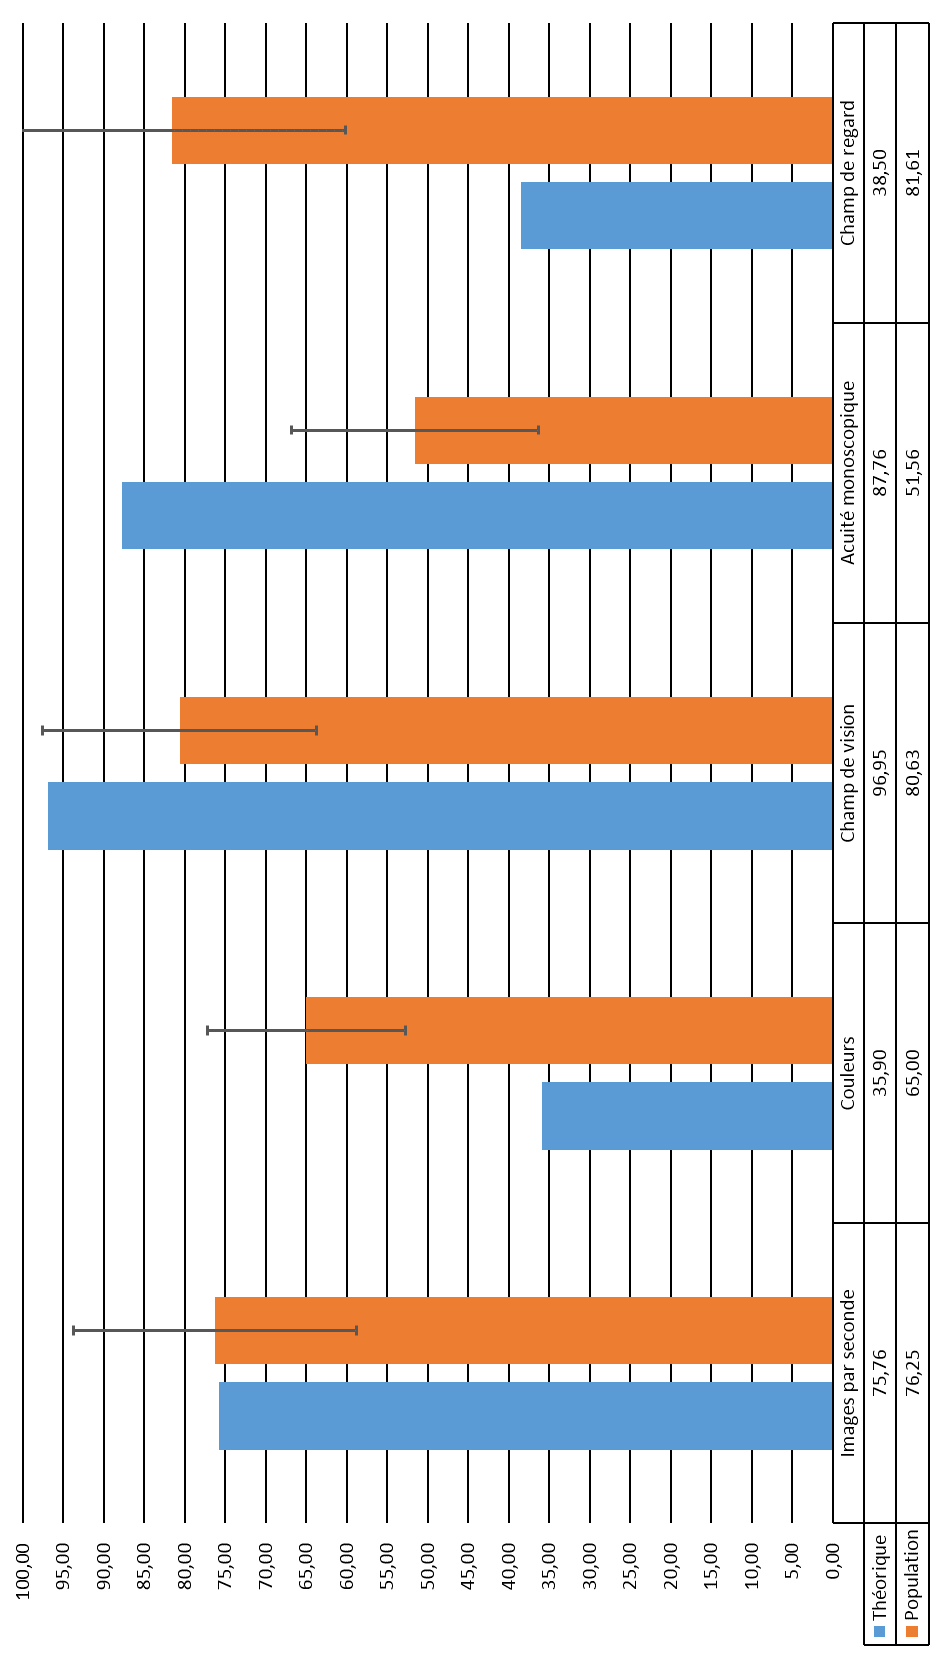
\includegraphics[scale=.75]{Figures/ResultsComparison}
		\caption{Résultats des valeurs théoriques calculées et des valeurs subjectives relevées.}
		\label{fig:results_comparison}
	\end{figure}
	
	\section{Discussion}
	\par Les résultats de la comparaison entre le modèle théorique et l'acceptation psychologique par les sujets peuvent être divisés en trois catégories. Premièrement les valeurs relevées sur les questionnaires correspondent plutôt bien aux valeurs données par le score théorique. C'est le cas par exemple pour le critère <<~images par seconde~>>.
	
	\par Deuxièmement, et en opposition à la première catégorie de résultats, deux critères diffèrent fortement par rapport aux valeurs d'acceptation par les sujets: dans un sens (pour les <<~couleurs~>> les valeurs subjectives sont supérieures aux valeurs objectives) comme dans l'autre (pour l'<<~acuité monoscopique~>> les valeurs théoriques sont supérieures aux valeurs d'acceptation).
	
	\par Enfin, la troisième catégorie contient des critères qui ont des valeurs objectives très différentes (96,95 pour le  <<~Champ de Vision~>> et un pauvre 38,50 pour le <<~Champ de Regard~>>) mais qui ont pourtant des valeurs subjectives très proches l'une de l'autre.   
	
	\subsection{Couleurs et acuité monoscopique}
	\par Ces deux critères montrent une grande différence de notation entre leur score théorique et leur score subjectif même si, à l'intérieur des sous catégories, les moyennes et les écarts-type sont assez proches.
	
	\par D'un côté, les sujets étaient globalement satisfaits de la quantité de couleurs bien que ce soit en fait assez peu par rapport à toutes les couleurs visible réellement. Une raison possible à cette divergence est l'absence de référence au monde réel pour juger par comparaison et l'utilisation massive d'appareils utilisant le même espace limité de couleurs (smartphones, télévisions, cinéma, ...).
	
	\par De l'autre côté, l'acuité monoscopique n'a pas été bien notée alors qu'elle aurait du paraitre suffisante. On peut l'expliquer aussi par l'habitude d'avoir une très forte demande sur la résolution des écrans, que ce soit pour les téléphones, les ordinateurs ou les écrans divers.
	
	\subsection{Champ de vision \& champ de regard}
	\par Bien que légèrement plus élevée, la valeur théorique du champ de vision est assez proche de sa valeur d'acception associée et est, en plus, contenue dans la majorité des écarts-type des sous catégories. Cependant, la valeur théorique du champ de regard est extrêmement basse comparée à sa valeur d'acceptation et éloignée de tous les écarts-type des sous-populations.
	
	\par La valeur théorique basse vient du fait que, même si l'angle de vision horizontal est très bon, il n'y a pas de face supérieure ce qui joue très négativement dans la notation de l'axe vertical du critère. A cause de la pondération quasi équivalente pour les deux axes, la note globale du critère est tirée vers le bas par la partie verticale qui est très basse.
	
	\par La tâche de conduite nécessite la quasi totalité de l'attention du conducteur à l'avant de la voiture et implique majoritairement l'axe horizontal de la vision. C'est pourquoi les sujets n'ont pas eu besoin d'utiliser particulièrement d'autres écrans que celui face à eux ni besoin d'images qui seraient hors-écrans. Cela peut expliquer pourquoi les participants ont noté le champ de regard si proche du champ de vision, car ils ont rarement dépassé les bornes du champ de vision et, quand c'était le cas, seulement un petit peu. Cela implique, dans ce cas précis, que notre hypothèse de pondération des axes en fonction de leur taille respective n'est pas correcte. Un jeu de pondération spécifique à la conduite devrait être calculé et appliqué, limitant considérablement l'influence de l'axe vertical.
	
	\par Enfin, on remarque une tendance intéressante à mettre en avant (bien que non soutenue par une preuve statistique). Les femmes (joueuses ou non) semblent être plus sévère dans leur notation que les hommes, et ce, quelle que soit la note théorique associée.